\documentclass[conference]{IEEEtran}
\IEEEoverridecommandlockouts

\usepackage{cite}
\usepackage{amsmath,amssymb,amsfonts}
\usepackage{graphicx}
\usepackage{array}
\usepackage{url}

\graphicspath{{figures/}}

% second row of author blocks
\makeatletter
\newcommand{\linebreakand}{%
  \end{@IEEEauthorhalign}
  \hfill\mbox{}\par
  \mbox{}\hfill\begin{@IEEEauthorhalign}
}
\makeatother

\begin{document}

\title{Optimization of Semiconductor Supply Chain Networks}

\author{
\IEEEauthorblockN{Aksaya Kanthan K S}
\IEEEauthorblockA{\textit{Amrita School of Artificial Intelligence,}\\
\textit{Coimbatore,}\\
\textit{Amrita Vishwa Vidyapeetham,}\\
India.\\
cb.ai.u4aid23003@cb.students.amrita.edu}
\and
\IEEEauthorblockN{Kiruthik Nandhan Murthi}
\IEEEauthorblockA{\textit{Amrita School of Artificial Intelligence,}\\
\textit{Coimbatore,}\\
\textit{Amrita Vishwa Vidyapeetham,}\\
India.\\
cb.ai.u4aid23018@cb.students.amrita.edu}
\and
\IEEEauthorblockN{Manasa V}
\IEEEauthorblockA{\textit{Amrita School of Artificial Intelligence,}\\
\textit{Coimbatore,}\\
\textit{Amrita Vishwa Vidyapeetham,}\\
India.\\
cb.ai.u4aid23022@cb.students.amrita.edu}
\linebreakand
\IEEEauthorblockN{Rithvik Rajesh}
\IEEEauthorblockA{\textit{Amrita School of Artificial Intelligence,}\\
\textit{Coimbatore,}\\
\textit{Amrita Vishwa Vidyapeetham,}\\
India.\\
cb.ai.u4aid23032@cb.students.amrita.edu}
\and
\IEEEauthorblockN{Shyam A V}
\IEEEauthorblockA{\textit{Amrita School of Business,}\\
\textit{Coimbatore,}\\
\textit{Amrita Vishwa Vidyapeetham,}\\
India.\\
av\_shyam@cb.amrita.edu}
}

\maketitle

\begin{abstract}
Outbound logistics in a semiconductor supply chain requires every customer order to be assigned a warehouse, an origin port and a carrier while respecting warehouse capacity, product availability, customer restrictions and the freight lanes that carriers actually serve. This paper presents a two-model Operations Research framework for these decisions, built on a public dataset of 9,215 orders of a global microchip producer. The seven dataset tables are joined to generate every feasible warehouse--port--carrier route of each order, and each route is priced with weight-banded freight rates and minimum charges. A maximum-flow test determines the shortest planning horizon in which the daily warehouse capacities can serve all orders. The first model is a binary integer programme that minimises the total warehouse and transportation cost. The second model is a weighted goal programme that balances total cost against average delivery time. Both models are solved exactly with the HiGHS solver. The minimum-cost plan serves all orders for \$15,517,994 over a seven-day horizon, and the goal programme reduces the average transit time from 2.64 days to 1.00 day for a cost increase of 0.22\%. Sensitivity analysis shows that demand volume and warehouse unit cost drive the total cost, whereas warehouse capacity changes the planning horizon rather than the cost. The models are delivered through an interactive web application that also plans single orders and uploaded batches of new orders, either on their own or together with the existing orders.
\end{abstract}

\begin{IEEEkeywords}
Supply Chain Optimization, Integer Programming, Goal Programming, Maximum Flow, Sensitivity Analysis, Logistics Network, Decision Support System
\end{IEEEkeywords}

\section{Introduction}
A global microchip producer fulfils thousands of customer orders through an outbound logistics network of warehouses, origin ports and transportation carriers. Each order can usually be shipped in several ways, but not in every way: a warehouse must stock the ordered product, some warehouses serve only specific customers, a warehouse is connected to only a few ports, and a carrier offers rates only on certain lanes and weight ranges. Warehouses also differ widely in storage cost and in the number of orders they can process per day.

In the historical data almost all volume is concentrated on one warehouse, one port and a small number of carriers. The data record what was done, not what was optimal. Because one order can have hundreds of feasible routes and all orders compete for the same warehouse capacity, the cheapest feasible plan cannot be read off the data and has to be found by optimisation.

This study formulates the problem as two sequential Operations Research models. The first model assigns exactly one feasible route to every order so that the total logistics cost is minimised subject to warehouse capacity. The second model keeps the same decisions and constraints and adds a delivery-time goal, so that the trade-off between cost and speed can be measured. Each model is then re-solved under perturbed capacity, cost, freight and demand parameters to study the robustness of the plan.

The models are implemented in a web application that parses the dataset, generates the feasible routes, solves both models and presents the plans, the trade-off curve and the sensitivity results. The application also contains a route planner for a single order and a bulk planner for an uploaded batch of orders.

\section{Dataset Details}
The Supply Chain Logistics Problem dataset \cite{dataset,dzalbs} is a publicly available real-world dataset describing the outbound logistics of a global microchip producer. It covers customer orders across the company's warehouse and port network and consists of seven related tables, summarised in Table~\ref{tab:tables}.

\begin{table}[htbp]
\caption{Tables of the Supply Chain Logistics Dataset}
\label{tab:tables}
\centering
\renewcommand{\arraystretch}{1.2}
\begin{tabular}{|l|r|p{0.52\columnwidth}|}
\hline
\textbf{Table} & \textbf{Rows} & \textbf{Description} \\
\hline
OrderList & 9,215 & Customer demand: product, customer, quantity, weight and service level. \\
\hline
FreightRates & 1,540 & Carrier lane rates by weight band, service level and mode, with minimum charge and transit days. \\
\hline
WhCosts & 19 & Storage cost per unit at each warehouse. \\
\hline
WhCapacities & 19 & Daily order-handling capacity of each warehouse. \\
\hline
ProductsPerPlant & 2,036 & Products that each warehouse is able to ship. \\
\hline
VmiCustomers & 14 & Customers to which specific warehouses are restricted. \\
\hline
PlantPorts & 22 & Warehouse to origin-port connectivity. \\
\hline
\end{tabular}
\end{table}

The order list contains 9,215 orders from 46 customers for 772 products. The network has 19 warehouses, 11 origin ports and one destination port, with 22 warehouse-to-port connections. Freight is offered by nine carriers over air and ground modes.

Each order has one of three service levels. Door-to-Port (DTP) orders, 6,218 in number, and Door-to-Door (DTD) orders, 2,143 in number, are shipped at the company's expense. For the 854 Customer Referred Freight (CRF) orders the customer arranges the freight, so the company decides only the warehouse and origin port and incurs only the warehouse cost.

Warehouse storage cost ranges from \$0.37 to \$2.04 per unit, and daily capacity ranges from 7 to more than 1,000 orders per day, for a total of 5,791 orders per day across the network. Transit times in the freight table range from 0 to 14 days.

The order list alone cannot be optimised, because the cost, feasibility and capacity information is held in the other six tables. Every join between the tables therefore acts as a feasibility filter on the routes an order may take.

\section{Methodology}

\subsection{Feasible Route Generation}
Let $O$ denote the set of orders and $P$ the set of warehouses. A route $r$ for order $o$ is a combination of a warehouse $p(r)$, an origin port, and, for DTD and DTP orders, a freight rate line that fixes the carrier, service and mode. A route is generated only if all of the following conditions hold:
\begin{itemize}
\item the warehouse stocks the ordered product (ProductsPerPlant);
\item the warehouse is permitted to serve the customer (VmiCustomers), where a warehouse absent from this table may serve any customer;
\item the warehouse is connected to the origin port (PlantPorts);
\item a freight rate exists from the origin port to the destination port whose weight band contains the order weight (FreightRates).
\end{itemize}
For CRF orders the last condition is not applied, since the customer arranges the freight. The resulting set of feasible routes of order $o$ is denoted
\begin{equation}
R_o = \{\, r : r \text{ satisfies all feasibility conditions for } o \,\}.
\end{equation}

Without the filters there are 17,333,415 order--warehouse--port--carrier combinations. After all joins 125,887 feasible routes remain, an average of 13.7 per order, and 7,387 orders can be served by only one warehouse. Fig.~\ref{fig:feasibility} shows this reduction.

\begin{figure}[htbp]
\centering
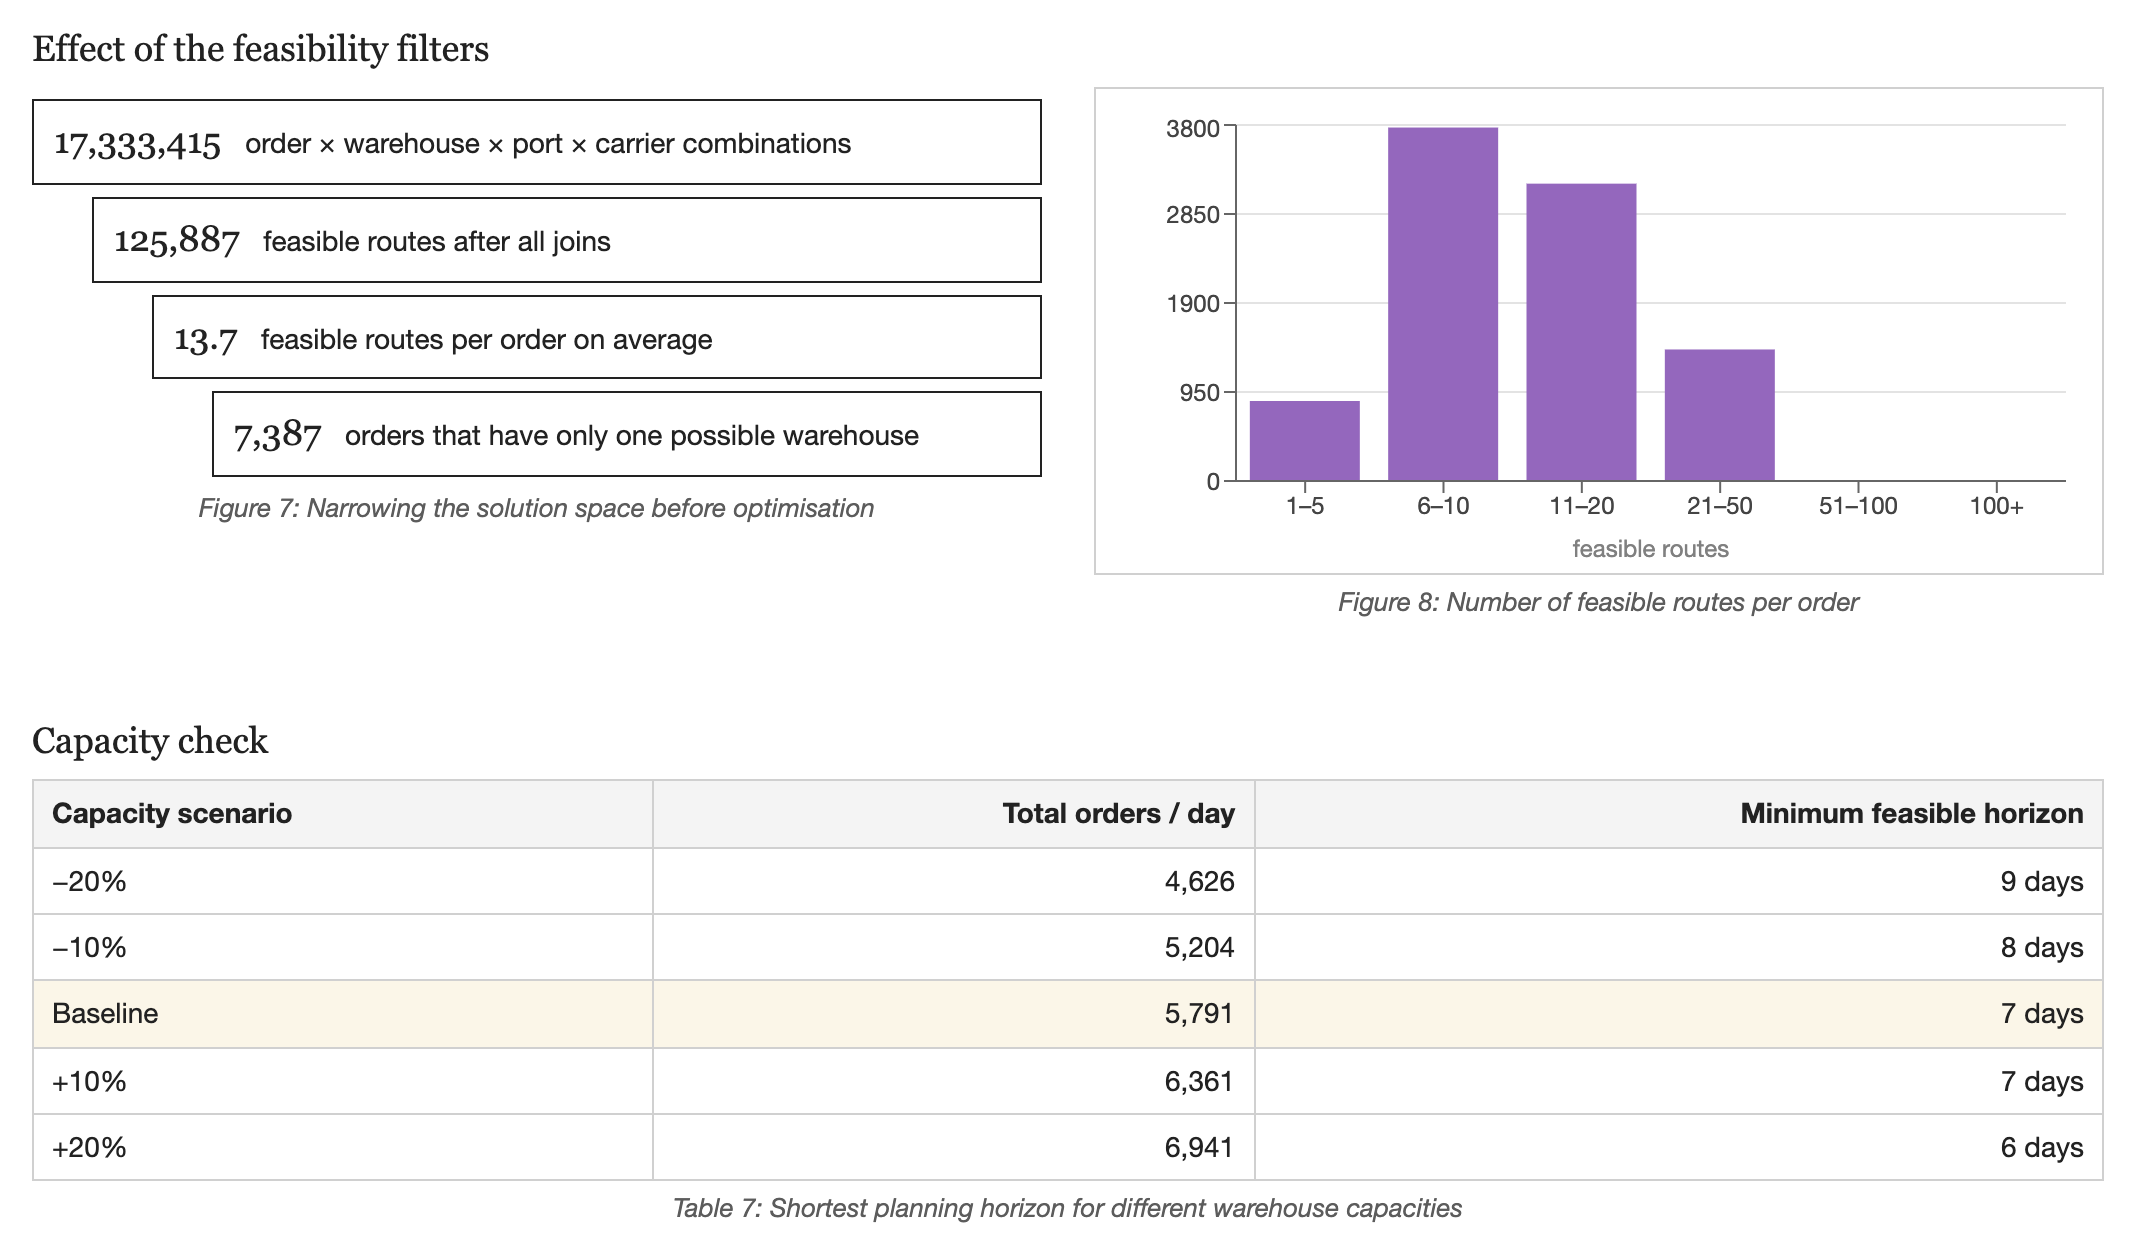
\includegraphics[width=\columnwidth]{feasibility.png}
\caption{Narrowing of the solution space by the feasibility filters, number of feasible routes per order, and the planning-horizon check.}
\label{fig:feasibility}
\end{figure}

\subsection{Route Cost}
Let $q_o$ and $w_o$ denote the unit quantity and weight of order $o$, $h_p$ the storage cost per unit at warehouse $p$, and $f_r$ and $m_r$ the rate and minimum charge of the freight line of route $r$. The warehouse cost of a route is
\begin{equation}
c^{W}_{or} = q_o \, h_{p(r)} ,
\end{equation}
and the transportation cost is the weight-based charge raised to the minimum charge:
\begin{equation}
c^{F}_{or} =
\begin{cases}
\max\left(m_r,\; w_o f_r\right), & \text{DTD and DTP orders},\\
0, & \text{CRF orders}.
\end{cases}
\end{equation}
The total cost of assigning route $r$ to order $o$ is
\begin{equation}
c_{or} = c^{W}_{or} + c^{F}_{or}.
\label{eq:cost}
\end{equation}
Because the weight band and the minimum charge are evaluated before optimisation, $c_{or}$ is a constant and the models remain linear.

\subsection{Planning Horizon}
Warehouse capacity is given in orders per day. Let $K_p$ denote the daily capacity of warehouse $p$ and $H$ the number of days in the planning horizon, so that warehouse $p$ can handle at most $H K_p$ orders. A horizon is feasible if every order can be assigned to one of its eligible warehouses within these limits.

Feasibility of a given $H$ is tested as a maximum-flow problem. A source is connected to every order with capacity one, every order is connected to its eligible warehouses with capacity one, and every warehouse is connected to a sink with capacity $H K_p$. The horizon is feasible if and only if the maximum flow equals $|O|$. The planning horizon is the smallest feasible value:
\begin{equation}
H^{*} = \min \left\{ H \in \mathbb{Z}_{>0} : \text{maxflow}(H) = |O| \right\}.
\end{equation}

Total capacity alone would suggest two days. However, warehouse PLANT03 is the only eligible warehouse for 6,868 orders and can process 1,013 orders per day, which forces $H^{*} = 7$ days. Both optimisation models therefore plan over a seven-day horizon.

\subsection{OR Model 1: Minimum-Cost Assignment}
The first model is a binary assignment model of the integer-programming type \cite{taha,hillier} that decides which feasible route serves each order. The decision variable is
\begin{equation}
x_{or} =
\begin{cases}
1, & \text{if order } o \text{ is shipped on route } r,\\
0, & \text{otherwise},
\end{cases}
\qquad r \in R_o .
\end{equation}

Every order must receive exactly one route:
\begin{equation}
\sum_{r \in R_o} x_{or} = 1, \qquad \forall\, o \in O .
\label{eq:demand}
\end{equation}
The orders assigned to a warehouse must not exceed its capacity over the horizon:
\begin{equation}
\sum_{o \in O} \; \sum_{\substack{r \in R_o \\ p(r) = p}} x_{or} \le H K_p, \qquad \forall\, p \in P .
\label{eq:capacity}
\end{equation}

The complete Model 1 formulation is
\begin{equation}
\begin{aligned}
\min_{x} \quad & Z_1 = \sum_{o \in O} \sum_{r \in R_o} c_{or}\, x_{or} \\
\text{s.t.} \quad & \sum_{r \in R_o} x_{or} = 1, && \forall\, o \in O, \\
& \sum_{o \in O} \; \sum_{\substack{r \in R_o \\ p(r) = p}} x_{or} \le H K_p, && \forall\, p \in P, \\
& x_{or} \in \{0, 1\}, && \forall\, o \in O,\; r \in R_o .
\end{aligned}
\label{eq:model1}
\end{equation}
Product availability, customer restrictions, port connectivity and freight lanes do not appear as constraints because routes that violate them are never generated.

The capacity constraint depends only on the warehouse of a route. For each order and warehouse, only the cheapest route can therefore appear in an optimal solution, and the other routes of that pair are removed before solving. This reduction is exact and makes the model considerably smaller.

\subsection{OR Model 2: Cost versus Delivery Time}
Model 1 ignores delivery time. Model 2 is a weighted goal programme \cite{ignizio} that retains the variables $x_{or}$ and the constraints \eqref{eq:demand} and \eqref{eq:capacity} and adds two goals with deviation variables.

Let $C^{*}$ denote the cost target, defined as the Model 1 optimum raised by an allowed budget percentage $\beta$:
\begin{equation}
C^{*} = (1 + \beta)\, Z_1^{*} .
\end{equation}
Let $t_r$ denote the transit days of route $r$, $N$ the number of DTD and DTP orders, and $T^{*}$ the target average transit time. CRF orders are excluded from the time goal because their transit is controlled by the customer.

The cost goal and the delivery-time goal are
\begin{equation}
\sum_{o \in O} \sum_{r \in R_o} c_{or}\, x_{or} - d_C^{+} + d_C^{-} = C^{*},
\label{eq:goalcost}
\end{equation}
\begin{equation}
\sum_{o \in O} \sum_{r \in R_o} t_r\, x_{or} - d_T^{+} + d_T^{-} = T^{*} N,
\label{eq:goaltime}
\end{equation}
where $d^{+} \ge 0$ and $d^{-} \ge 0$ are the over-achievement and under-achievement of each goal. Only over-achievement is undesirable, so the objective penalises $d_C^{+}$ and $d_T^{+}$. Each deviation is divided by its target so that money and days can be weighed together:
\begin{equation}
\min \quad Z_2 = w_C \frac{d_C^{+}}{C^{*}} + w_T \frac{d_T^{+}}{T^{*} N} + \varepsilon \frac{\sum_{o}\sum_{r} c_{or}\, x_{or}}{C^{*}} ,
\label{eq:model2}
\end{equation}
where $w_C$ and $w_T$ are the goal weights and $\varepsilon = 10^{-3}$ is a small tie-breaking term that selects the cheapest plan when both goals can be met.

The complete Model 2 minimises \eqref{eq:model2} subject to \eqref{eq:demand}, \eqref{eq:capacity}, \eqref{eq:goalcost}, \eqref{eq:goaltime}, $x_{or} \in \{0,1\}$ and non-negative deviation variables. For Model 2, a route is removed before solving only if another route of the same order and warehouse is both no more expensive and no slower. The default settings are $\beta = 5\%$, $T^{*} = 1$ day and $w_C = w_T = 1$.

\subsection{Solution Method}
Both models are solved with the HiGHS mixed-integer programming solver \cite{highs} using branch-and-bound with a relative optimality gap of 0.1\%. The feasible routes, weight-band prices and planning horizon are computed once and reused by both models and by every sensitivity scenario.

\subsection{Sensitivity Analysis}
Linear-programming shadow prices are not reliable for a model with binary variables. Each scenario is therefore solved again from scratch and compared with the unperturbed plan of the same model. The scenarios change one parameter at a time: warehouse capacity by $\pm 10\%$ and $\pm 20\%$, freight rates by $+10\%$ and $+20\%$, warehouse unit cost by $\pm 10\%$, and demand volume by $+10\%$ and $+20\%$, where a demand change scales both the quantity and the weight of every order so that weight bands are re-evaluated. For each scenario the planning horizon is recomputed, and the number of orders whose route differs from the baseline plan is recorded. For Model 2 the delivery-time target is additionally varied to trace the cost--time trade-off curve.

\subsection{Planning of New Orders}
Two further tools reuse the same feasibility filters. The route planner enumerates every feasible route of a single entered order and ranks the routes by cost, by transit time, or by cost plus a penalty per transit day. The bulk planner reads a file of new orders, rejects rows that cannot be routed together with the reason, and solves Model 1 for the remaining orders.

Both tools offer two planning scopes. In the first scope the new orders are planned on their own against the full warehouse capacities. In the second scope the new orders are appended to the existing orders and Model 1 is re-solved for all orders together, so that new and existing orders compete for the same capacity. The added cost, the change in planning horizon and the number of existing orders that are re-routed are then reported.

\section{Results and Discussion}

\subsection{Minimum-Cost Assignment}
Model 1 was solved over the seven-day horizon for all 9,215 orders. The solver returned an optimal plan in less than one second. The results are summarised in Table~\ref{tab:model1}.

\begin{table}[htbp]
\caption{Minimum-Cost Plan of OR Model 1}
\label{tab:model1}
\centering
\renewcommand{\arraystretch}{1.2}
\begin{tabular}{|l|r|}
\hline
\textbf{Measure} & \textbf{Value} \\
\hline
Planning horizon & 7 days \\
\hline
Total logistics cost & \$15,517,994 \\
\hline
Warehouse cost & \$15,489,878 \\
\hline
Transportation cost & \$28,116 \\
\hline
Average transit time (DTD and DTP orders) & 2.64 days \\
\hline
Warehouses used & 11 of 19 \\
\hline
Carriers used & 5 of 9 \\
\hline
\end{tabular}
\end{table}

Warehouse cost accounts for 99.8\% of the total cost, so the choice of warehouse affects the cost far more than the choice of carrier. Fig.~\ref{fig:p1load} shows the orders assigned to each warehouse against its seven-day capacity and the carriers selected for the DTD and DTP orders. PLANT03 receives 7,091 orders, which is exactly its seven-day capacity, and is the only binding capacity constraint. Every other warehouse has slack; for example, PLANT02 receives 640 orders against a capacity of 966. Carriers V444\_0 and V444\_1 carry most of the company-paid shipments.

\begin{figure}[htbp]
\centering
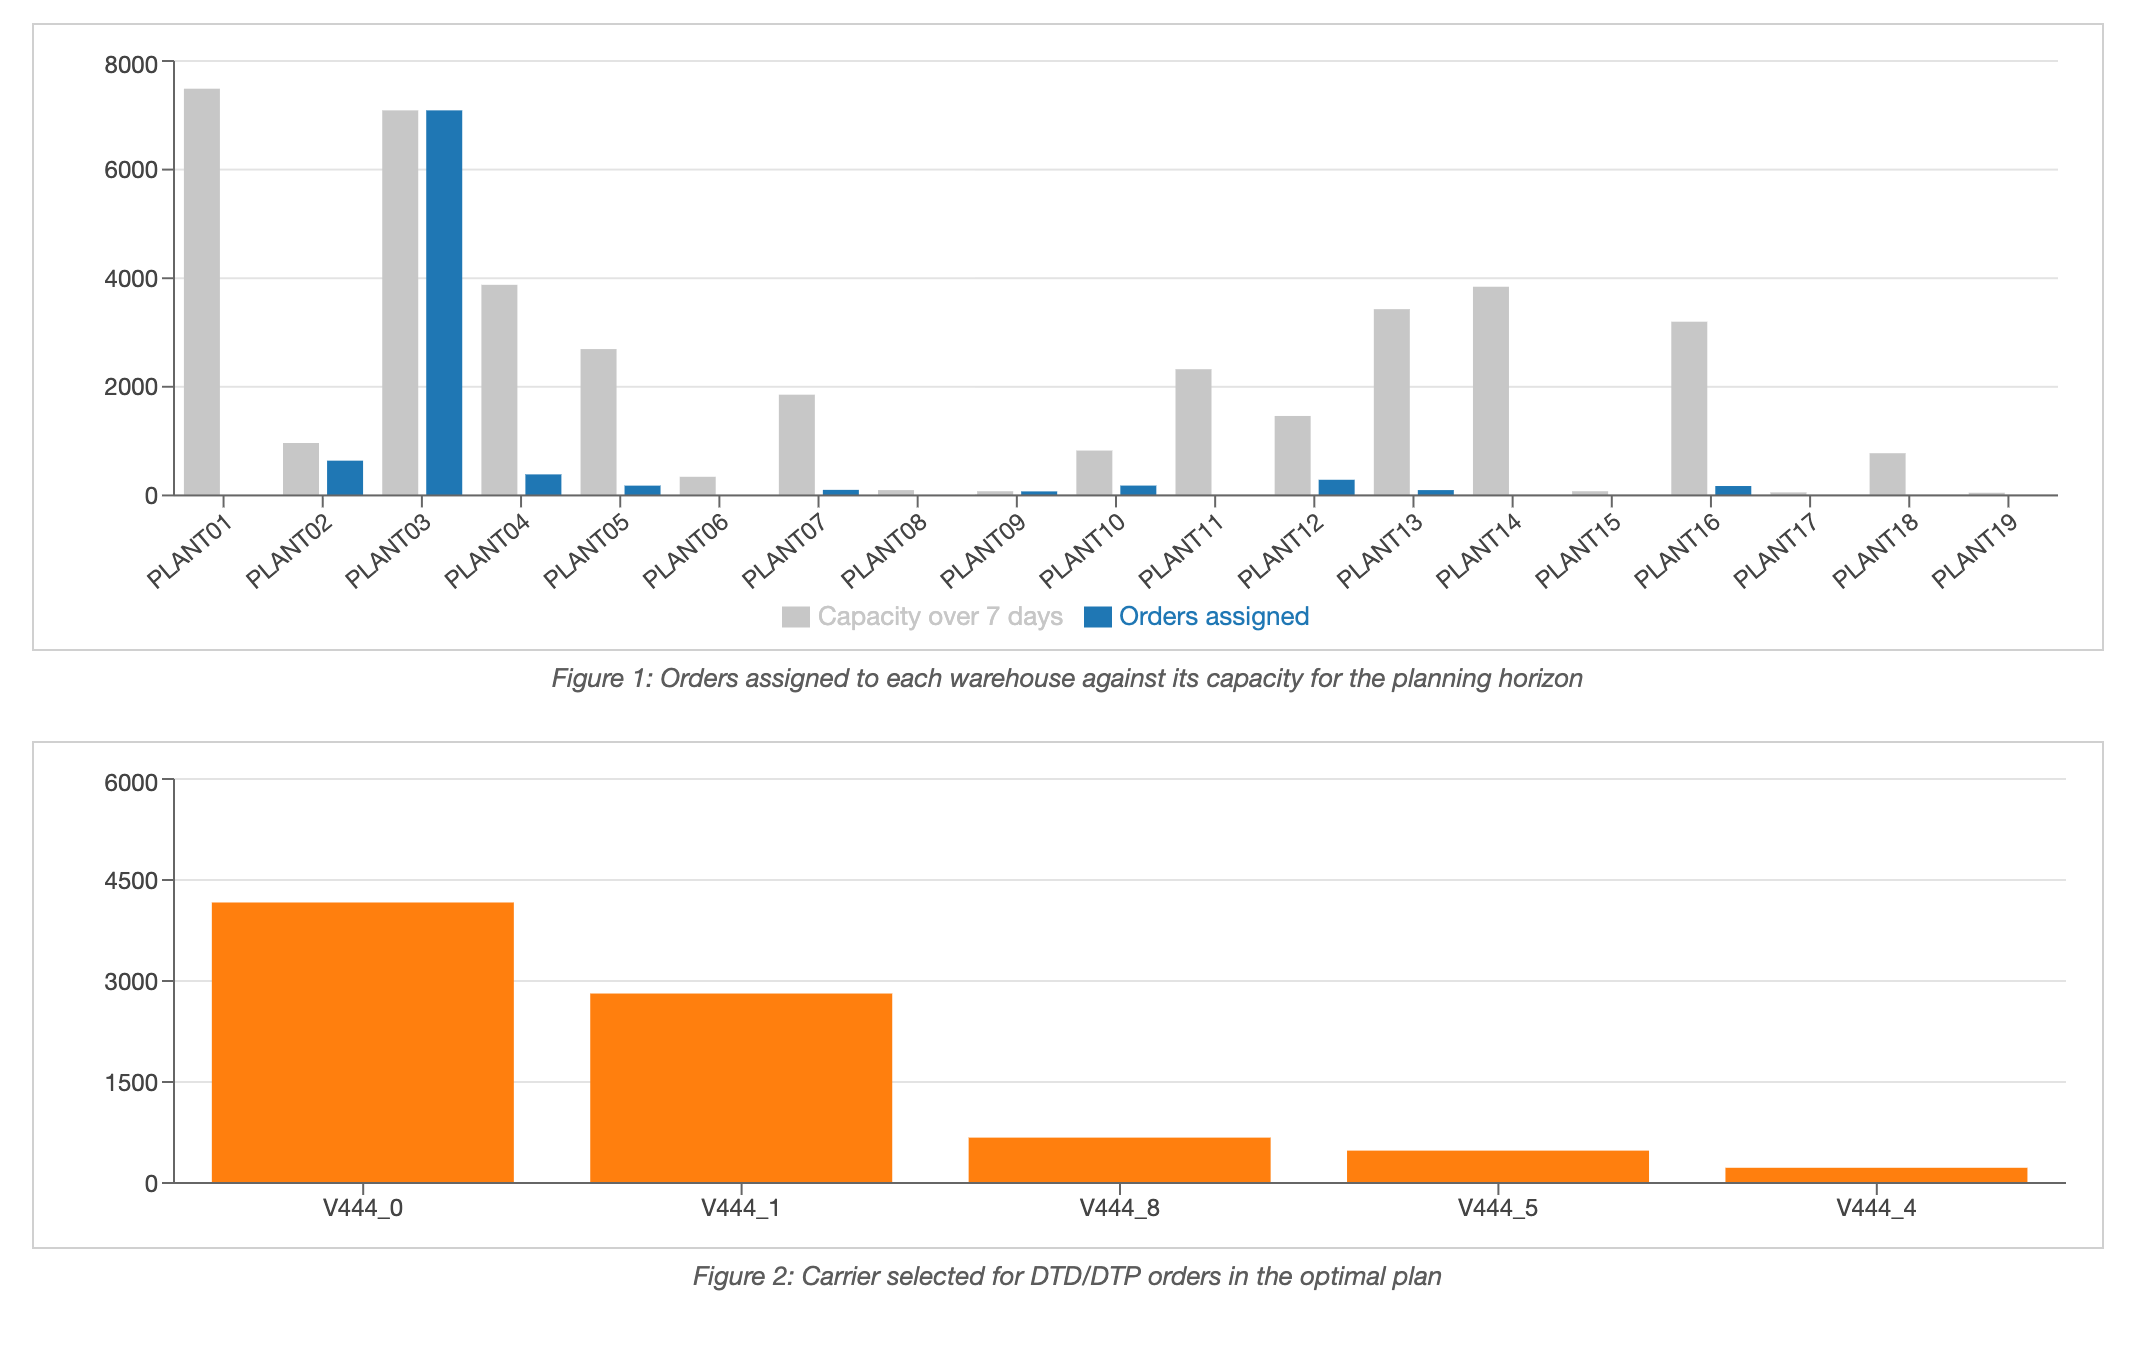
\includegraphics[width=\columnwidth]{p1_load.png}
\caption{Orders assigned to each warehouse against its seven-day capacity, and carriers selected for DTD and DTP orders, in the Model 1 plan.}
\label{fig:p1load}
\end{figure}

\subsection{Cost versus Delivery Time}
Model 2 was solved with the default goals: a cost target 5\% above the Model 1 optimum, that is \$16,293,893, and a target average transit time of one day, with equal weights. Both goals were met. Table~\ref{tab:compare} compares the two plans.

\begin{table}[htbp]
\caption{Comparison of OR Model 1 and OR Model 2}
\label{tab:compare}
\centering
\footnotesize
\setlength{\tabcolsep}{4pt}
\renewcommand{\arraystretch}{1.2}
\begin{tabular}{|l|r|r|r|}
\hline
\textbf{Measure} & \textbf{Model 1} & \textbf{Model 2} & \textbf{Change} \\
\hline
Total cost & \$15,517,994 & \$15,551,482 & $+0.22\%$ \\
\hline
Warehouse cost & \$15,489,878 & \$15,489,356 & $-0.003\%$ \\
\hline
Transportation cost & \$28,116 & \$62,126 & $+121\%$ \\
\hline
Average transit & 2.64 days & 1.00 day & $-62.1\%$ \\
\hline
Planning horizon & 7 days & 7 days & none \\
\hline
\end{tabular}
\end{table}

The average transit time falls from 2.64 days to 1.00 day for a cost increase of \$33,488, or 0.22\%. The faster delivery is obtained almost entirely by selecting faster carriers: the transportation cost more than doubles, but it remains a very small share of the total cost, while the warehouse assignment is nearly unchanged.

To measure how much each further gain in speed costs, the goal programme was re-solved for a range of delivery-time targets. The results are given in Table~\ref{tab:tradeoff} and Fig.~\ref{fig:tradeoff}.

\begin{table}[htbp]
\caption{Goal Programme Re-Solved for Different Delivery-Time Targets}
\label{tab:tradeoff}
\centering
\footnotesize
\setlength{\tabcolsep}{4pt}
\renewcommand{\arraystretch}{1.2}
\begin{tabular}{|r|r|r|r|}
\hline
\textbf{Target (days)} & \textbf{Achieved (days)} & \textbf{Total cost} & \textbf{vs Model 1} \\
\hline
0.25 & 0.25 & \$15,694,514 & $+1.14\%$ \\
\hline
0.50 & 0.50 & \$15,633,001 & $+0.74\%$ \\
\hline
1.00 & 1.00 & \$15,551,482 & $+0.22\%$ \\
\hline
1.50 & 1.50 & \$15,524,010 & $+0.04\%$ \\
\hline
2.00 & 2.00 & \$15,521,442 & $+0.02\%$ \\
\hline
3.00 & 2.64 & \$15,517,994 & $0.00\%$ \\
\hline
\end{tabular}
\end{table}

\begin{figure}[htbp]
\centering
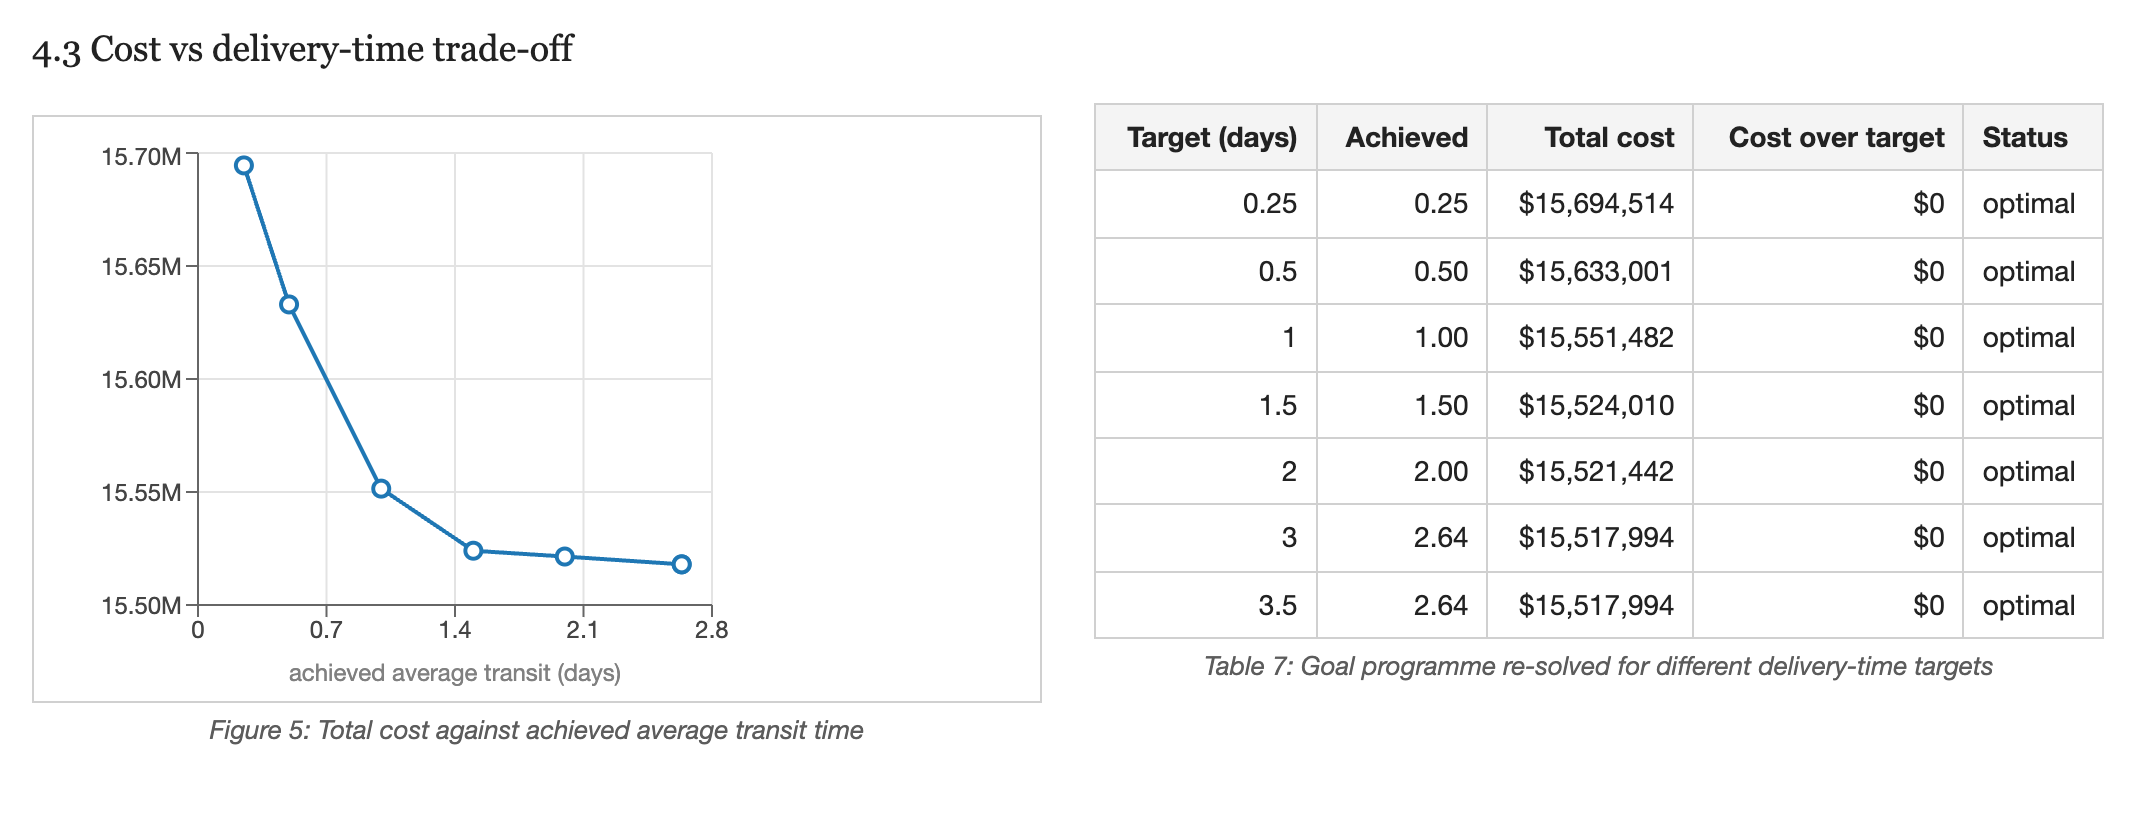
\includegraphics[width=\columnwidth]{p2_tradeoff.png}
\caption{Total logistics cost against the achieved average transit time for different delivery-time targets.}
\label{fig:tradeoff}
\end{figure}

The trade-off curve is convex: each further reduction in transit time costs more than the previous one. Reducing the average transit to about one day costs 0.22\%, whereas reaching 0.25 days costs 1.14\%. When the target is looser than 2.64 days the goal programme returns the minimum-cost plan of Model 1.

\subsection{Sensitivity Analysis}
Table~\ref{tab:sensitivity} reports the Model 1 plan re-optimised under each parameter change, and Fig.~\ref{fig:sensitivity} shows the corresponding change in total cost.

\begin{table}[htbp]
\caption{Sensitivity of the Model 1 Plan to Parameter Changes}
\label{tab:sensitivity}
\centering
\footnotesize
\setlength{\tabcolsep}{4pt}
\renewcommand{\arraystretch}{1.2}
\begin{tabular}{|l|c|r|r|r|}
\hline
\textbf{Scenario} & \textbf{Horizon} & \textbf{Total cost} & \textbf{Change} & \textbf{Re-routed} \\
\hline
Baseline & 7 d & \$15,517,994 & -- & 0 \\
\hline
Capacity $-20\%$ & 9 d & \$15,517,238 & $0.00\%$ & 199 \\
\hline
Capacity $-10\%$ & 8 d & \$15,517,246 & $0.00\%$ & 197 \\
\hline
Capacity $+10\%$ & 7 d & \$15,516,674 & $-0.01\%$ & 391 \\
\hline
Capacity $+20\%$ & 6 d & \$15,517,099 & $-0.01\%$ & 199 \\
\hline
Freight $+10\%$ & 7 d & \$15,520,805 & $+0.02\%$ & 0 \\
\hline
Freight $+20\%$ & 7 d & \$15,523,617 & $+0.04\%$ & 2 \\
\hline
Warehouse cost $-10\%$ & 7 d & \$13,969,006 & $-9.98\%$ & 0 \\
\hline
Warehouse cost $+10\%$ & 7 d & \$17,066,981 & $+9.98\%$ & 1 \\
\hline
Demand $+10\%$ & 7 d & \$17,067,529 & $+9.99\%$ & 225 \\
\hline
Demand $+20\%$ & 7 d & \$18,617,042 & $+19.97\%$ & 358 \\
\hline
\end{tabular}
\end{table}

\begin{figure}[htbp]
\centering
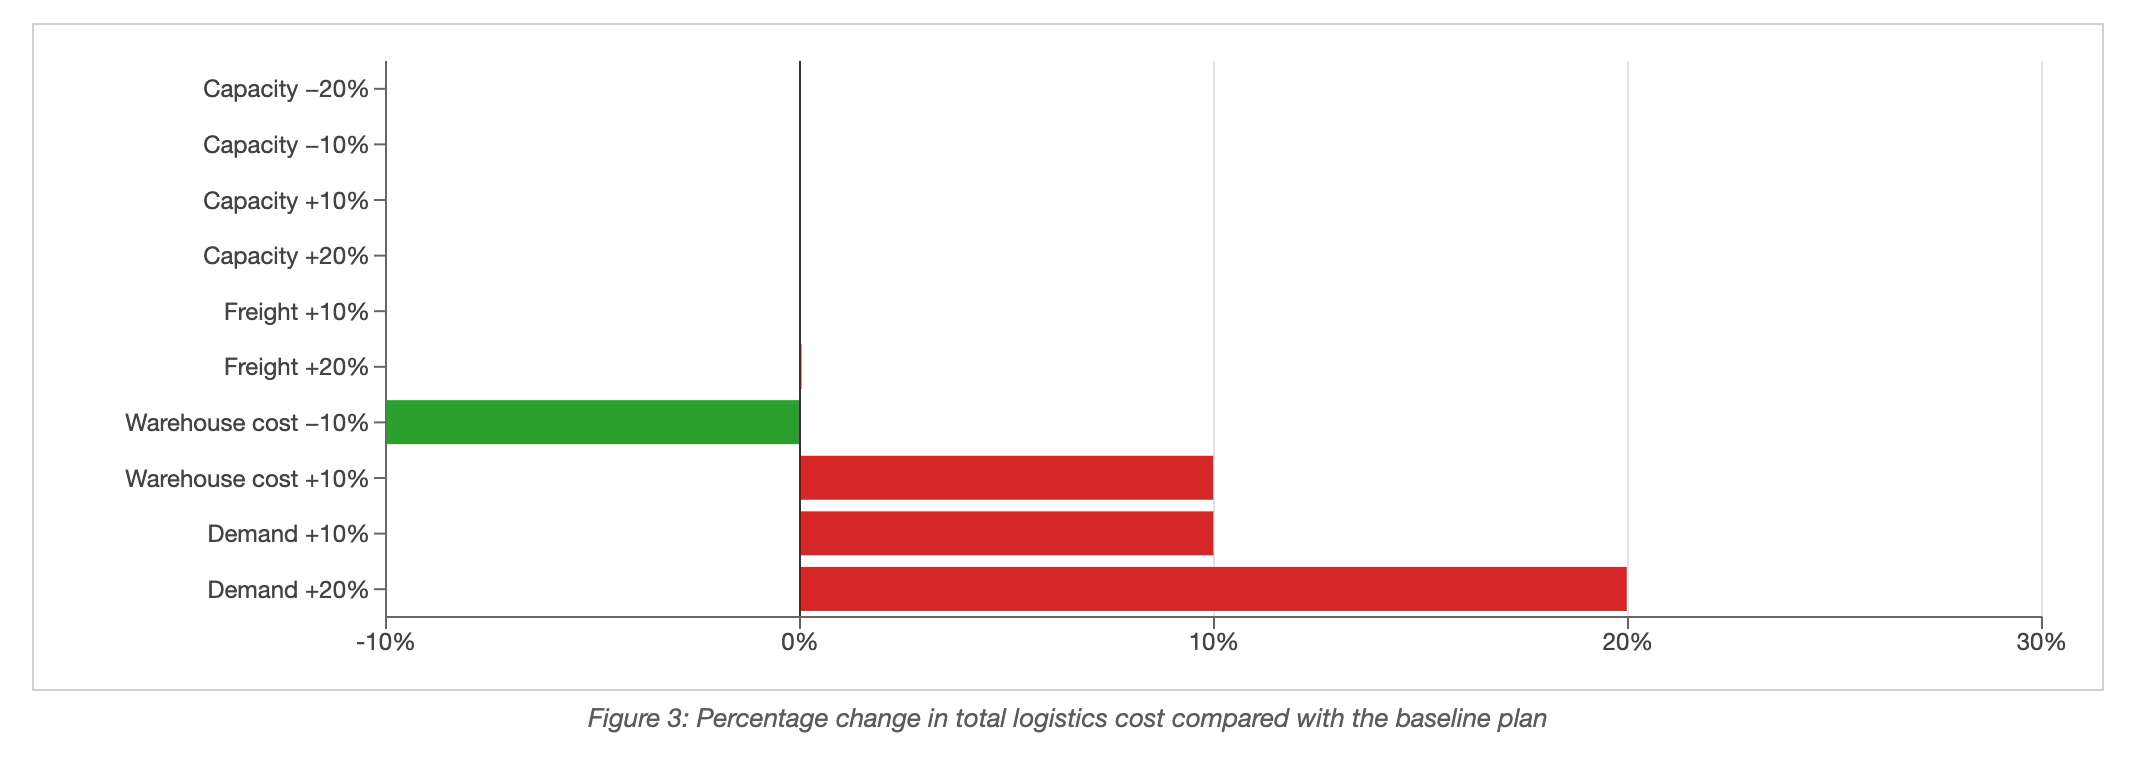
\includegraphics[width=\columnwidth]{p1_sensitivity.png}
\caption{Percentage change in total logistics cost of the Model 1 plan under each parameter change.}
\label{fig:sensitivity}
\end{figure}

Demand volume and warehouse unit cost have the largest influence: a 20\% demand surge raises the cost by 19.97\%, and a 10\% change in warehouse unit cost changes the total by 9.98\%. Freight rates have almost no influence, because transportation is only 0.2\% of the total cost. Changes in warehouse capacity leave the cost essentially unchanged but move the planning horizon, from six days at $+20\%$ capacity to nine days at $-20\%$, and re-route between 197 and 391 orders. Capacity therefore determines how quickly the orders can be served rather than how much they cost.

\subsection{Planning of New Orders}
Fig.~\ref{fig:planner} shows the route planner for a single DTP order. Of the 19 warehouses, three can serve the order, and 47 feasible routes are compared. The optimal route has a total cost of \$142.86 and is highlighted in the network of feasible options.

\begin{figure}[htbp]
\centering
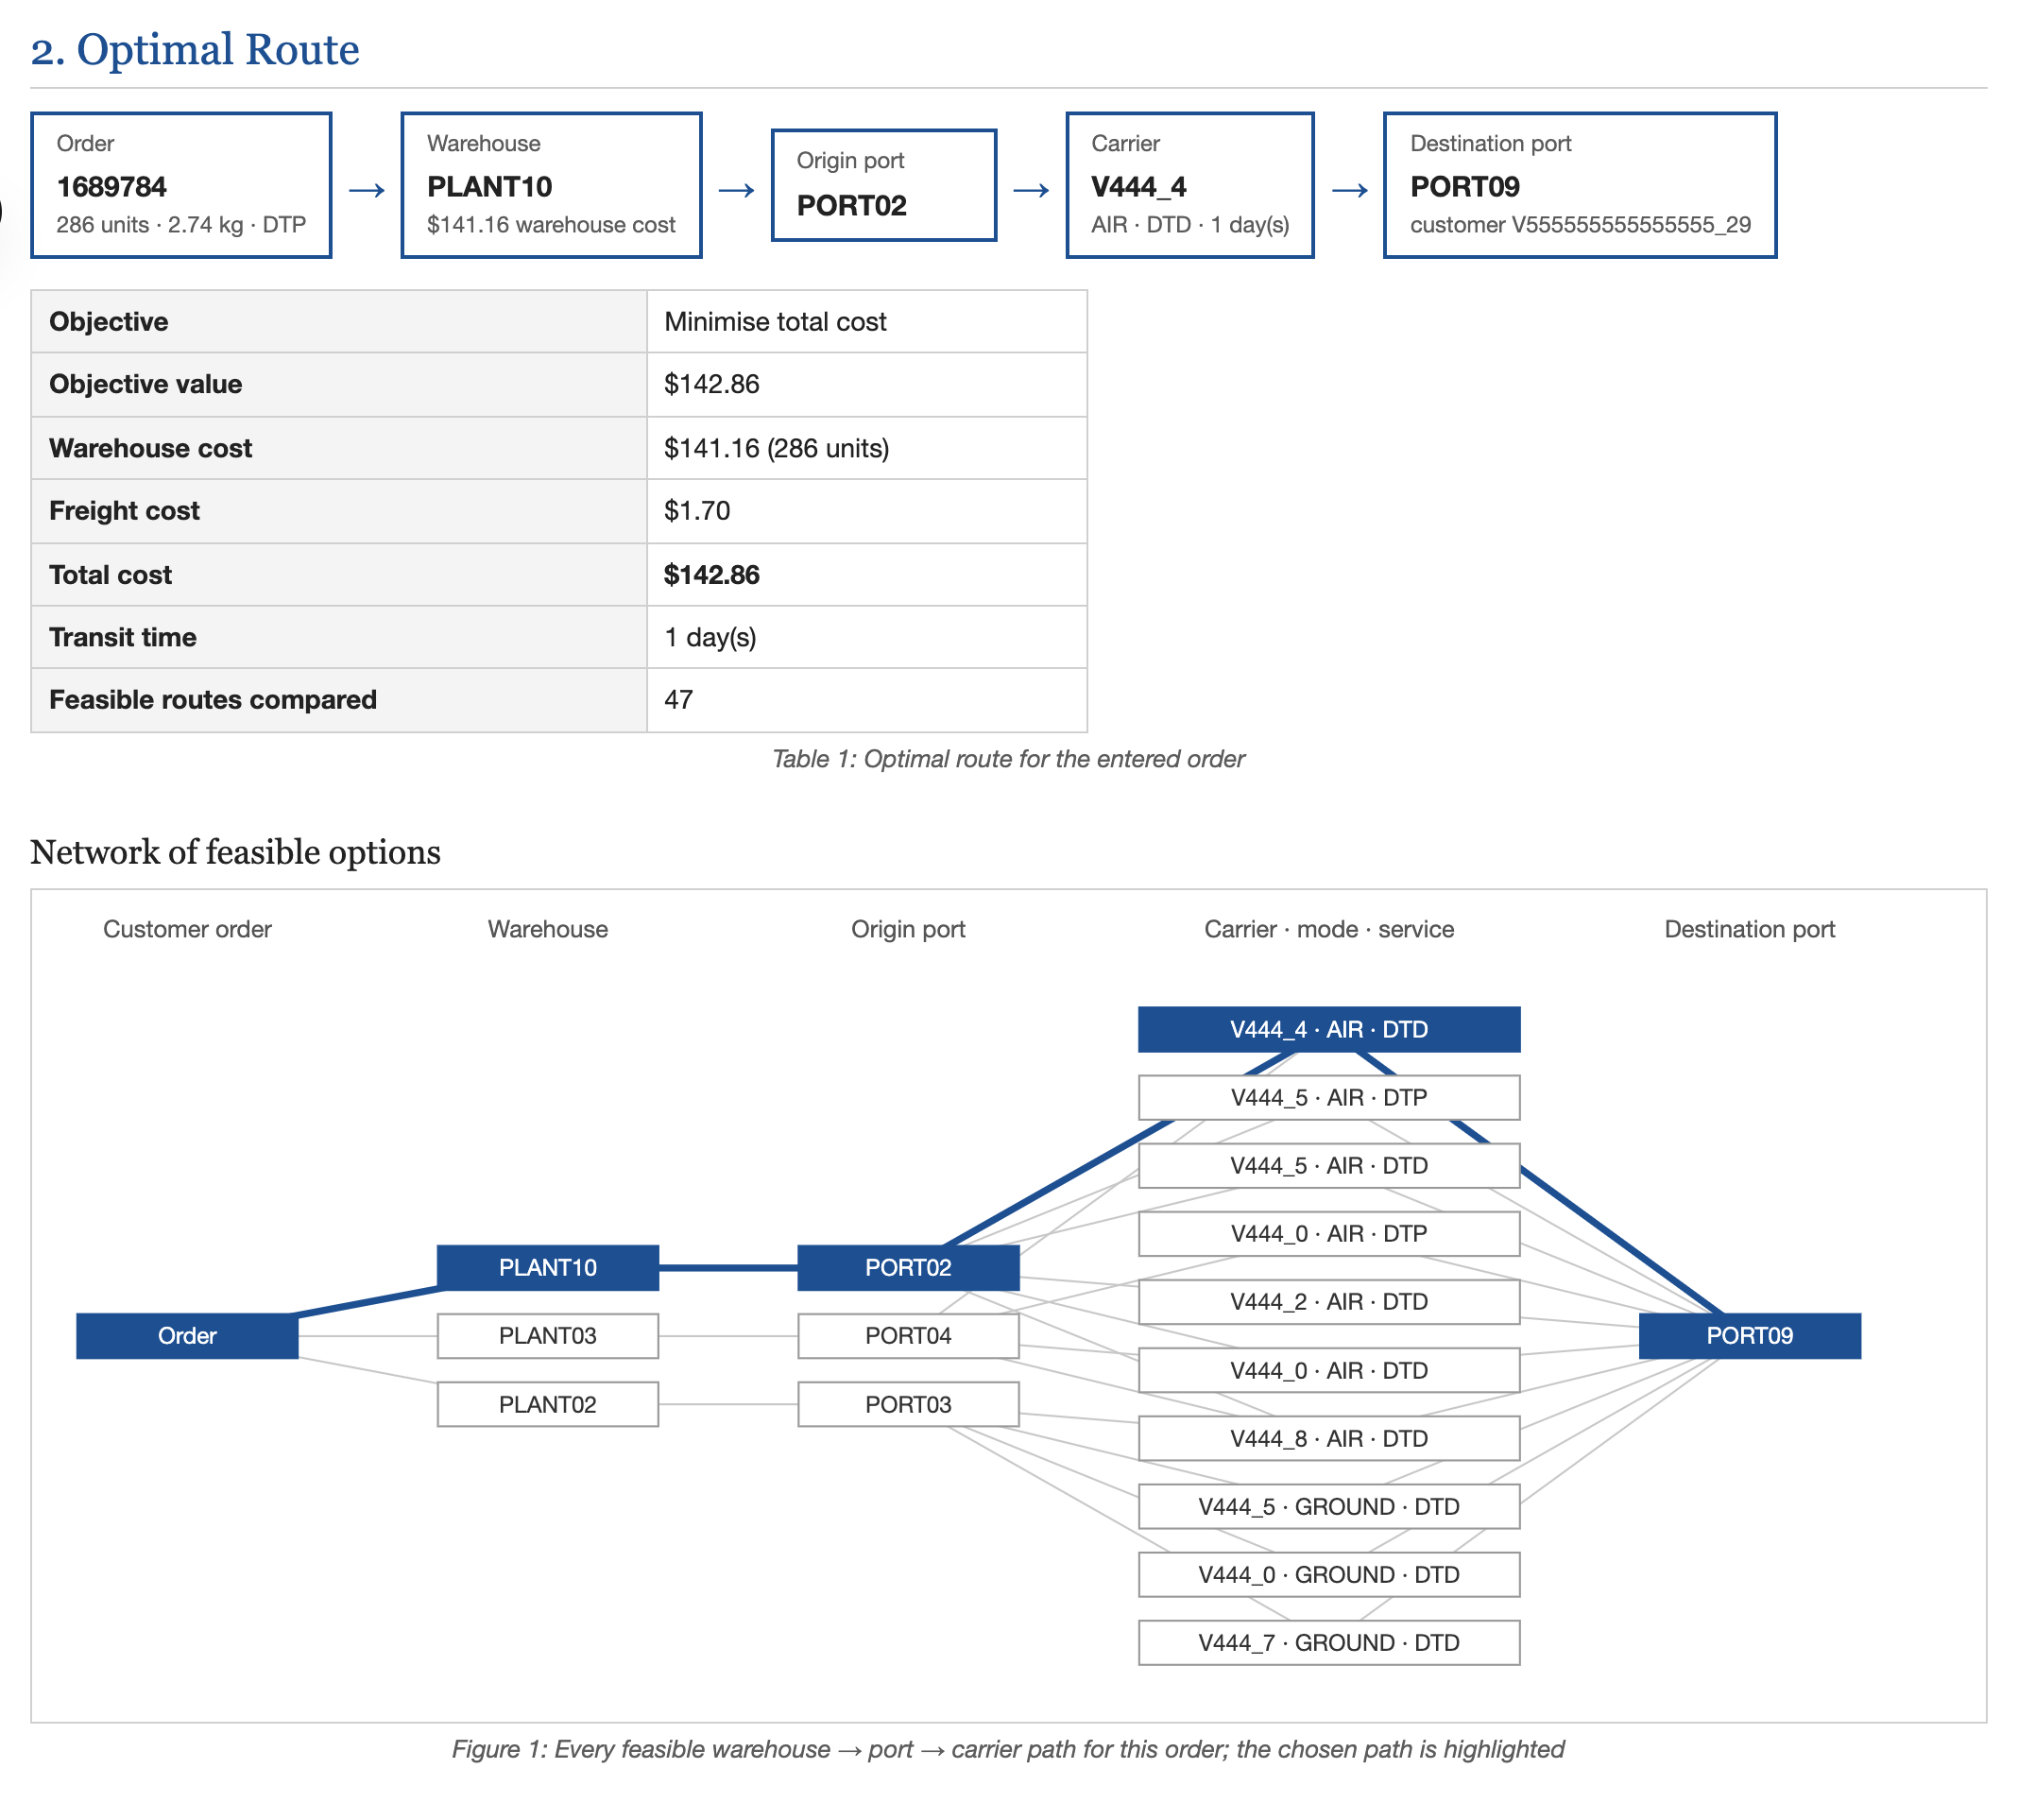
\includegraphics[width=\columnwidth]{planner.png}
\caption{Route planner: optimal route of a single order and the network of all feasible warehouse--port--carrier paths.}
\label{fig:planner}
\end{figure}

The bulk planner was tested with a file of 255 rows. Five rows were rejected, for an unknown product, an invalid service level, a missing weight, a weight outside every freight weight band and a repeated order identifier. The remaining 250 orders, planned on their own, cost \$541,478 over a one-day horizon.

When the same 250 orders are planned together with the 9,215 existing orders, Model 1 is re-solved for all 9,465 orders. The total cost rises from \$15,517,994 to \$16,060,720, an added cost of \$542,726, the horizon remains seven days, and 187 existing orders are moved to another warehouse to make room, as shown in Fig.~\ref{fig:bulk}. The added cost is \$1,248 higher than the cost of the batch planned alone, which is the price of the capacity that the new orders take from the existing plan.

\begin{figure}[htbp]
\centering
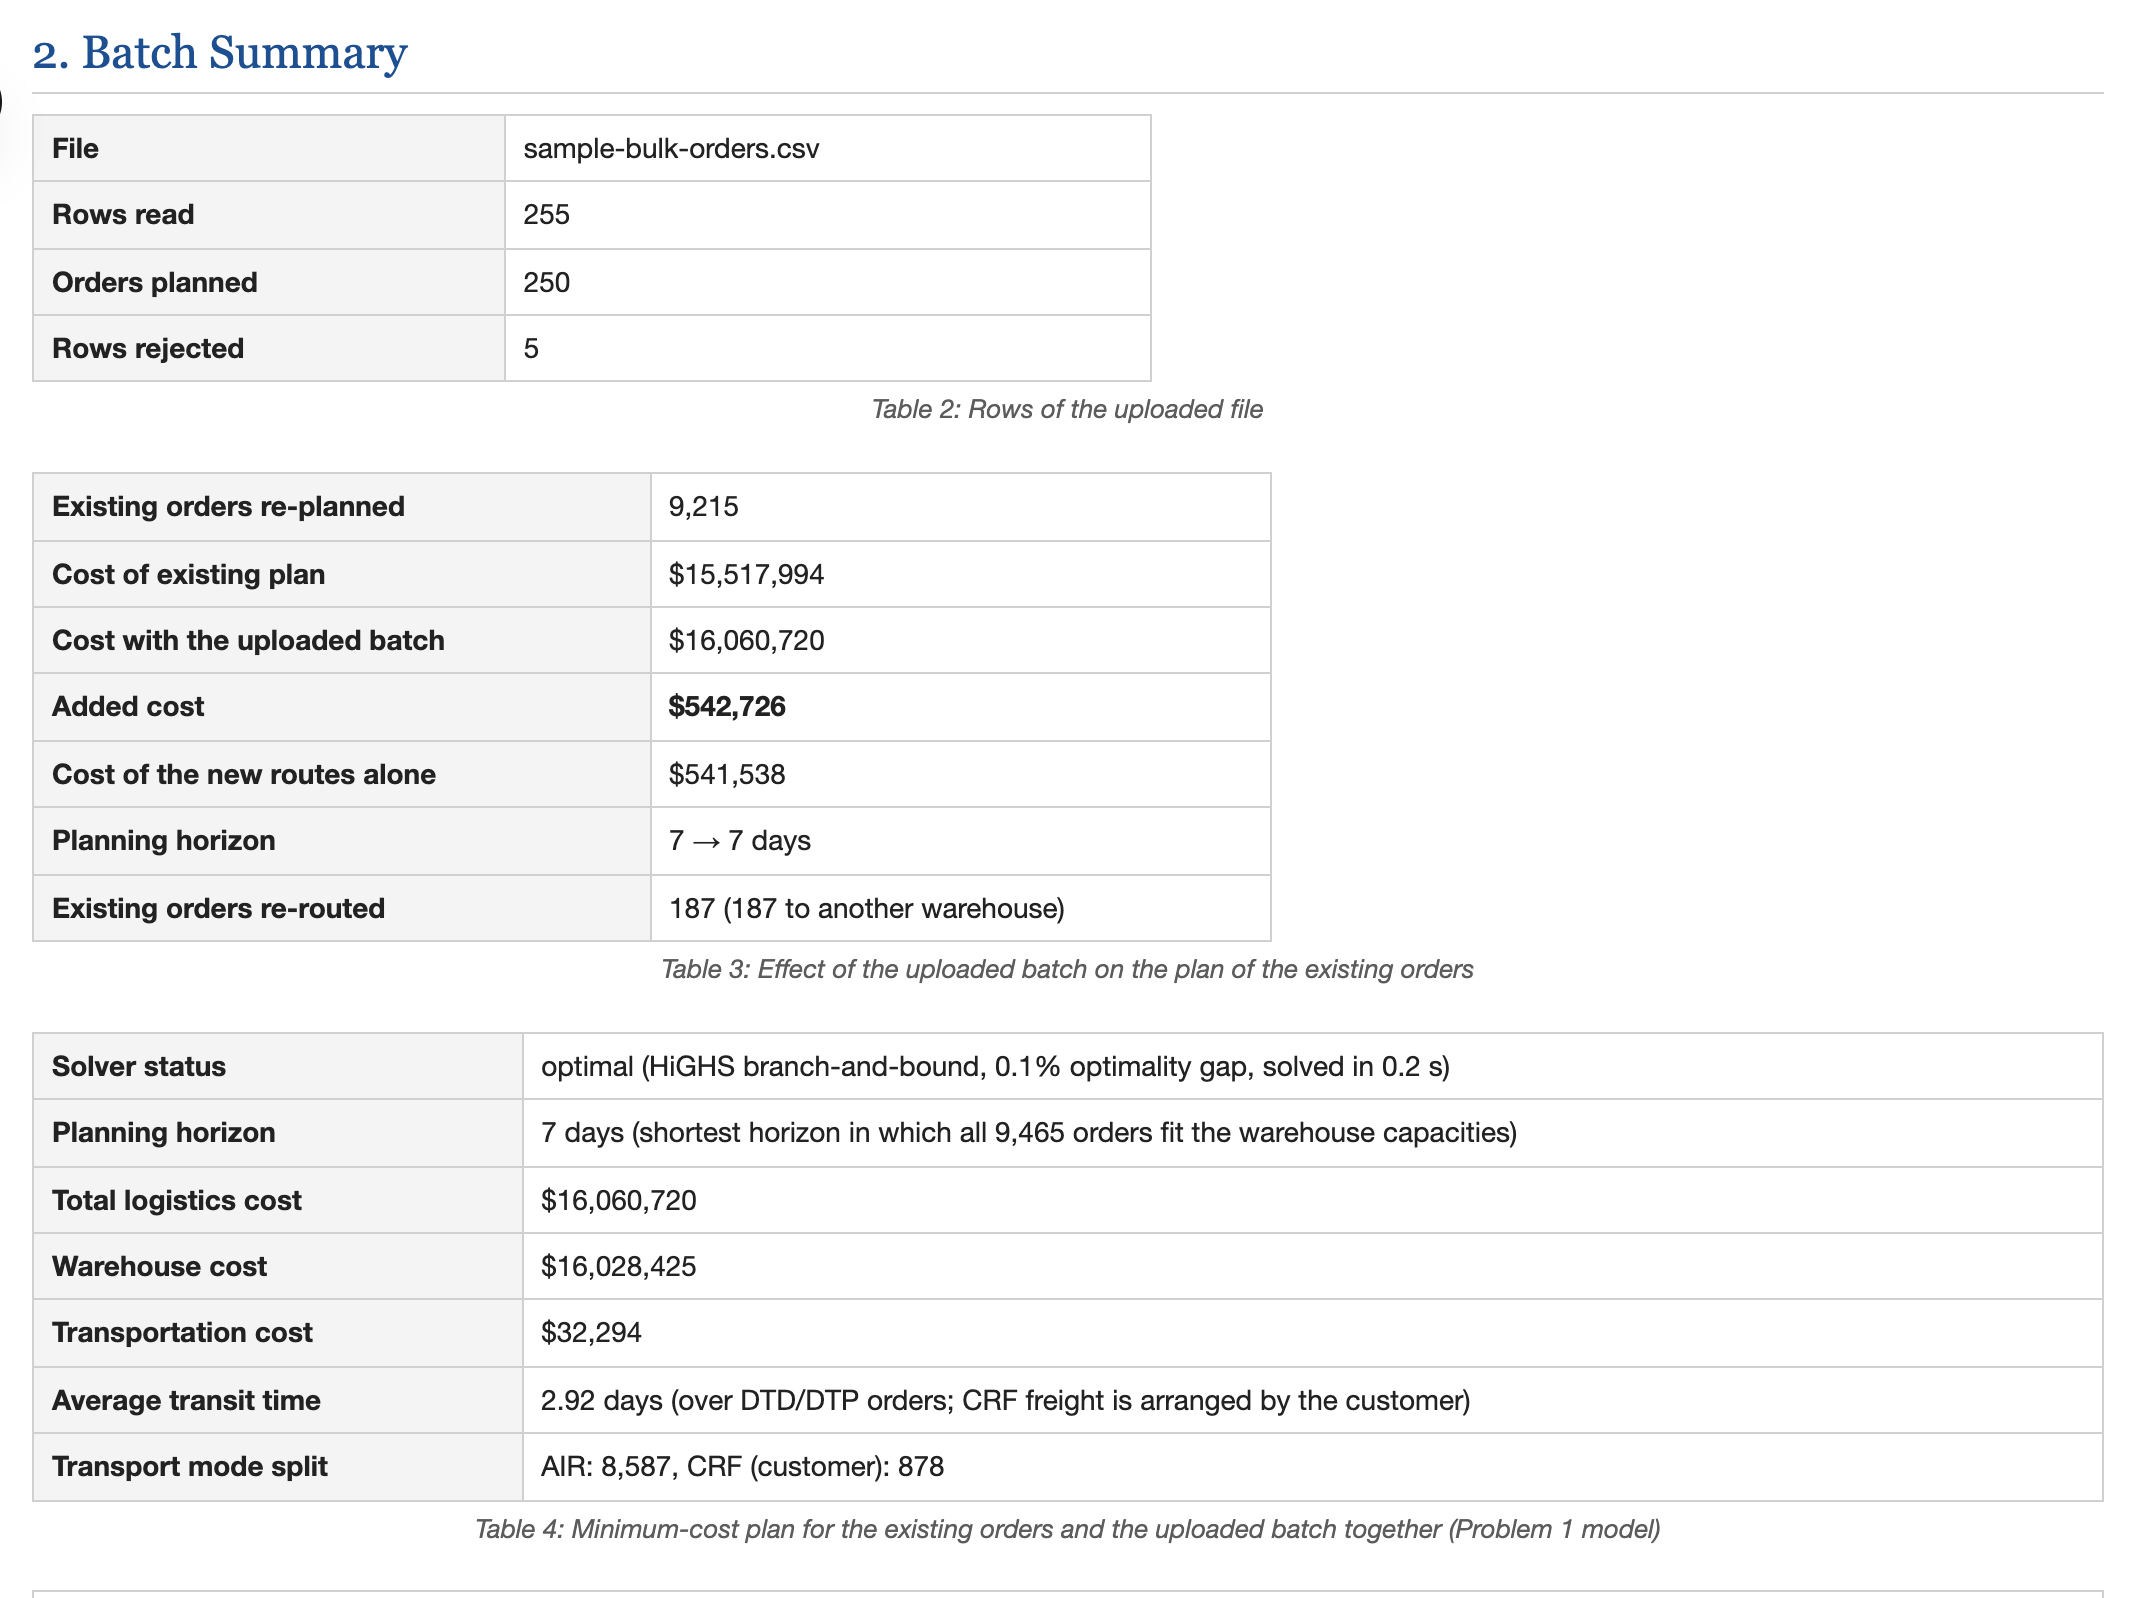
\includegraphics[width=\columnwidth]{bulk_combined.png}
\caption{Bulk planner: an uploaded batch of 250 orders re-planned together with the existing orders.}
\label{fig:bulk}
\end{figure}

\subsection{Decision Support Application}
The models are implemented in a web application built with Next.js and TypeScript. The server parses the dataset workbook, generates and prices the feasible routes, builds the integer and goal programmes and solves them with the WebAssembly build of HiGHS. The interface is organised into five tabs: dataset analysis, the two optimisation models with their sensitivity analyses, the route planner and the bulk planner. The decisions made by the solver, namely the warehouse, origin port, carrier and mode, are highlighted in every result table so that a plan can be read without reference to the mathematical formulation.

\section{Conclusion}
This study presented a two-model Operations Research framework for the outbound logistics of a semiconductor supply chain. The seven tables of a public dataset were joined to generate the feasible warehouse--port--carrier routes of 9,215 orders, which reduced more than 17 million combinations to 125,887 feasible routes. A maximum-flow test showed that a single warehouse, which is the only option for most orders, forces a seven-day planning horizon.

The first model formulated the assignment of routes to orders as a binary integer programme that minimises warehouse and transportation cost under warehouse capacity. The optimal plan costs \$15,517,994, of which 99.8\% is warehouse cost, and uses 11 of the 19 warehouses and 5 of the 9 carriers.

The second model added cost and delivery-time goals to the same decisions. With the default goals the average transit time is reduced from 2.64 days to 1.00 day for a cost increase of 0.22\%, and the trade-off curve shows that further gains in speed become progressively more expensive.

Sensitivity analysis showed that the total cost is driven by demand volume and warehouse unit cost, that freight rates have little effect, and that warehouse capacity determines the planning horizon rather than the cost.

The framework can be extended in future work by deciding which warehouses should be active at all through a facility-location model, by consolidating shipments, by ranking carriers on qualitative criteria with the Analytic Hierarchy Process, and by modelling volume discounts and other nonlinear cost relationships.

\begin{thebibliography}{00}
\bibitem{dataset} T. Kalganova and I. Dzalbs, ``Supply Chain Logistics Problem Dataset,'' Brunel University London, 2019. [Online]. Available: \url{https://doi.org/10.17633/rd.brunel.7558679.v2}
\bibitem{dzalbs} I. Dzalbs and T. Kalganova, ``Accelerating supply chains with Ant Colony Optimization across a range of hardware solutions,'' \textit{Computers \& Industrial Engineering}, vol. 147, Art. no. 106610, 2020, doi: 10.1016/j.cie.2020.106610.
\bibitem{highs} Q. Huangfu and J. A. J. Hall, ``Parallelizing the dual revised simplex method,'' \textit{Mathematical Programming Computation}, vol. 10, no. 1, pp. 119--142, 2018.
\bibitem{taha} H. A. Taha, \textit{Operations Research: An Introduction}, 10th ed. Pearson, 2017.
\bibitem{hillier} F. S. Hillier and G. J. Lieberman, \textit{Introduction to Operations Research}, 10th ed. McGraw-Hill, 2015.
\bibitem{ignizio} J. P. Ignizio, \textit{Goal Programming and Extensions}. Lexington Books, 1976.
\end{thebibliography}

\end{document}
